%%% 特別研究報告書サンプル
\documentclass[dvipdfmx]{ampbt_nomag}

%%% クラスオプション:
%%% chapter: \chapterコマンドを使用可能にする(jsbook (report) を使う).
%%% その他 jsclasses に指定可能なオプションが指定できます(そのまま渡される).

%%% 題目 %%%%%%%%%%%%%%%%%%%%%%%%%%%%%%%%%%%%%%%%%%%%%%%%%%%%%%%%%%%%%%%%%%%%%%%%
\title{模倣学習による
}     % 題目1行目
      {修士論文生成手法の検討}                             % 題目2行目
      {}                                             % 題目3行目
%%% 指導教員 %%%%%%%%%%%%%%%%%%%%%%%%%%%%%%%%%%%%%%%%%%%%%%%%%%%%%%%%%%%%%%%%%%%%
\supervisors{森本淳}{教授}    % 指導教員1人目 {氏名}{職名}
            {}{}    % 指導教員2人目 {氏名}{職名}
            {}{}                % 指導教員3人目 {氏名}{職名}
%%% 入学年月 %%%%%%%%%%%%%%%%%%%%%%%%%%%%%%%%%%%%%%%%%%%%%%%%%%%%%%%%%%%%%%%%%%%%
\entrancedate{2022}{4}          % {年}{月}
%%% 著者氏名 %%%%%%%%%%%%%%%%%%%%%%%%%%%%%%%%%%%%%%%%%%%%%%%%%%%%%%%%%%%%%%%%%%%%
\author{古巻}{鉄平}             % {姓}{名}
%%% 提出日 %%%%%%%%%%%%%%%%%%%%%%%%%%%%%%%%%%%%%%%%%%%%%%%%%%%%%%%%%%%%%%%%%%%%%%
\submissiondate{2024}{2}{5}    % {年}{月}{日}
%%% 背表紙の幅 %%%%%%%%%%%%%%%%%%%%%%%%%%%%%%%%%%%%%%%%%%%%%%%%%%%%%%%%%%%%%%%%%%
\setlength{\wdspine}{15mm}
%%% 背表紙の出力枚数 %%%%%%%%%%%%%%%%%%%%%%%%%%%%%%%%%%%%%%%%%%%%%%%%%%%%%%%%%%%%
\def\numberofspines{1}
%%% 摘要 %%%%%%%%%%%%%%%%%%%%%%%%%%%%%%%%%%%%%%%%%%%%%%%%%%%%%%%%%%%%%%%%%%%%%%%%
\abstract{%
}
%%% パッケージの読み込みや自分用のマクロの定義 %%%%%%%%%%%%%%%%%%%%%%%%%%%%%%%%%%
\usepackage{amsmath,amssymb}
\usepackage{algorithmic}
\usepackage{algorithm}
\usepackage{graphicx}
\usepackage[subrefformat=parens]{subcaption}


%%%\usepackage{bxpapersize} %%%消すべき?
\newcommand{\rme}{\mathrm{e}}
\renewcommand{\bfdefault}{bx}


%%% 出力の制御 %%%%%%%%%%%%%%%%%%%%%%%%%%%%%%%%%%%%%%%%%%%%%%%%%%%%%%%%%%%%%%%%%%

%%% 本文を出力しない場合,次の行のコメントを外して下さい.
%%\outputbodyfalse

%%% 末尾に表紙,背表紙を出力しない場合,次の行のコメントを外して下さい.
%% \outputcoverfalse

%%% 末尾に提出用摘要を出力しない場合,次の行のコメントを外して下さい.
%% \outputabstractforsubmissionfalse

%%% ampbt.cls では表紙等の作成のために geometry パッケージを使用しているため,本文
%%% のレイアウトを変えるために \usepackage[...]{geometry} とすると Option clash が
%%% 発生します.何らかの理由で本文のレイアウトを変更したい場合は \geometry{...} を
%%% 使用して下さい.
%%% また,jsclasses を使用しているため,例えば 3cm を指定したい場合は 3truecm と書
%%% く必要があります.
%% \geometry{hmargin=3truecm,vmargin=2truecm}

\begin{document}
\ifoutputbody
%%% 中表紙,摘要,目次 %%%%%%%%%%%%%%%%%%%%%%%%%%%%%%%%%%%%%%%%%%%%%%%%%%%%%%%%%%
\makeinsidecover                % 中表紙
\makeabstract                   % 摘要
\maketoc                        % 目次
\setcounter{page}{1}            % 本文のページ番号を1から始める
%%% 本文 %%%%%%%%%%%%%%%%%%%%%%%%%%%%%%%%%%%%%%%%%%%%%%%%%%%%%%%%%%%%%%%%%%%%%%%%
\section{序論}\label{sec-intro}		% 本文の開始
人間の手を模倣した多指ハンドロボットの実用化は社会的に大きな意義がある.人間が日常生活を送るにあたって手で物体を操るという動作は必要不可欠であるが,多指ハンドロボットが実現することでこれらの動作を代替することができる.このような多指ハンドロボットには,多種多様な形状を持つ物体を操る能力が要求される.これまで様々な多指ハンドロボットの開発が進められてきたものの,多指ハンドロボットを人間のように器用に動かす制御手法については依然として開発が進んでおらず実用化とは程遠い状況にある.\\
%%% 「このような多指ハンドロボットには,多種多様な形状を持つ物体を操る能力が要求される.」という文章はどこかには絶対欲しいが場所を間違えている気がする.
多指ハンドロボットの制御手法の開発では,操作する物体との間に接触が多くモデル化が困難である点が特に問題となる.このような課題を解決するため,多指ハンドロボットの制御手法としてモデルフリー強化学習がよく用いられる.モデルフリー強化学習では力学モデルの存在を陽に仮定せず,環境との相互作用を繰り返すことによって制御方策を獲得する\cite{RLBook}.一方で,モデルフリー強化学習は複雑なタスクの学習を可能にしたものの,あるタスクを学習して得られた方策を環境のわずかに異なる別のタスクに適用するのは困難である\cite{hua2021learning}.このため,多指ハンドロボットの目的である様々な形状の物体の操作を達成することが出来ない.\\
%%% 「環境」「タスク」という用語を突然登場させないほうが良い?
このようなモデルフリー強化学習の課題を解決するために(12月8日ミーティングでの話を考慮して書く.「階層強化学習」ではない.「オプション」「downstream task」あたりの話をまとめて書く.)
\\
本研究ではこのような〜〜〜を用いて複数の形状のバルブを短時間で学習させる.\\
(実験結果)\\


\section{関連研究}\label{sec-related_papers}
%%% オプションやdownstreamの話を入れ込む形で修正する.
\subsection{スキルを用いた強化学習}
事前に収集したデータから複数のタスクの学習を効率化するための手段として,スキルの事前学習が研究されている.スキルの事前学習では,情報が付加されていないデータを収集し,そのデータからスキルを抽出する.その後,抽出したスキルを行動として利用することで学習する.Singhらは,正規化フロー法\cite{dinh2016density}を用いて標準正規分布に従うノイズベクトルを行動ベクトルへ射影することで,学習速度を向上させる行動の事前分布を獲得した\cite{singh2020parrot}.また,Pertschらは,事前に収集したデータから行動の系列をサンプリングし,変分オートエンコーダ(VAE)によってサンプリングした系列の再構成学習を行うことで,スキルを潜在空間上に埋め込み高速な学習を実現する手法を開発した\cite{pertsch2021accelerating}.本研究では事前に収集したデータからスキルを抽出することでハンドロボットの回転タスクについて,未知のタスクに対する学習速度を向上させる手法を検討する.

\subsection{多指ハンドロボット}
・多指ハンドロボットは古くから開発されてきた.\\
  ・ワイヤ駆動のロボット:Shadow Adroit\cite{kumar2014real}\\
  ・Direct-drivenなどロボット:Allegro\\
・しかし,これらのロボットは費用が高く,故障時の修理が困難である.\\
%%% もう一種類挙げたい.
・近年は低価格かつ修理が容易なトイロボットであるRobel\cite{ahn2020robel},LEAP hand\cite{shaw2023leap}などが強化学習の研究に用いられている.\\
%%% LEAP handは最近出たばかりなので強化学習の研究によく用いられるではおかしい.
%%% 接触センサの話は不要?博士の研究を視野に入れるなら...?

\subsection{多指ハンドロボットの低次元制御}

\subsection{接触の多いタスクの制御}
・強化学習を用いている研究をいくつか\\
・目的は,現状どこまで出来ているかを明らかにすること.\\
・OpenAIのルービックキューブの研究など.\\

\section{手法}\label{sec-method}
\subsection{強化学習(整理し直す)}
本研究ではロボットの制御問題をマルコフ決定過程$\mathcal{M} = (\mathcal{S},\mathcal{A},p,r)$によってモデリングする.$\mathcal{S}$,$\mathcal{A}$はそれぞれ状態空間,行動空間を意味しており,現在の状態$s_t \in \mathcal{S}$で行動$a_t \in \mathcal{A}$をとった時に状態$s_{t+1}\in\mathcal{S}$へと遷移する状態遷移確率を$ p:\mathcal{S}\times\mathcal{A}\times\mathcal{S}\rightarrow[0,1]$,この時エージェントが得る報酬を $r:\mathcal{S}\times\mathcal{A}\rightarrow\mathbb{R}$と表す.また,方策$\pi(a_t|s_t)$に従って行動した際に得られる状態と行動の系列において,$s_t$が表れる確率を$\rho_\pi(s_t)$,$s_t$と$a_t$が同時に表れる確率を$\rho_\pi(s_t,a_t)$,デモンストレーションデータの中に$s_t$と$a_t$が同時に現れる確率を$\rho_D(s_t,a_t)$ と表記する.\\
通常の強化学習では,累積報酬$\sum_t \mathbb{E}_{(s_t,a_t)\sim\rho_\pi}[r(s_t, a_t)]$を最大化することを目指す.ただし,実際はステップ数が無限大の時に発散しないために割引率$\gamma$を$r$の前にかけることが多い.累積報酬の最大化に向け,まず各状態における状態価値関数と行動を含めた行動価値関数を以下のように定義する.
\begin{eqnarray} \label{state_value1}
  V_\pi(s) &=& \mathbb{E}_{\rho_\pi} \left[\sum^{\infty}_{k=0}\gamma^kr(s_{t+k},a_{t+k}) \middle|s_t = s\right] \\
  \label{state_value2}
  Q_\pi(s,a) &=& \mathbb{E}_{\rho_\pi} \left[\sum^{\infty}_{k=0}\gamma^kr(s_{t+k},a_{t+k}) \middle|s_t = s, a_t = a \right]
\end{eqnarray}
この時,式(\ref{state_value1})を
\begin{eqnarray} \label{bellman_equation}
  V_\pi(s) &=& \mathbb{E}_{\rho_\pi} \left[ r(s_t,a_t) + \sum^{\infty}_{k=1} \gamma^{k}r(s_{t+k},a_{t+k}) \middle|s_t = s\right] \\ \nonumber
  &=& \mathbb{E}_{\rho_\pi} \left[ r(s_t,a_t) + \gamma V_\pi(s_{t+1}) \middle|s_t = s\right]
\end{eqnarray}
のように変形することでベルマン方程式が得られる.式(\ref{bellman_equation})における期待値をとる操作を最大値をとる操作に置き換えたものをベルマン最適方程式と呼び,期待値をとるものはベルマン期待方程式と呼ぶ.このベルマン方程式の右辺を$V_\pi(\cdot)$の写像と見做すことで次のようなベルマン作用素$\mathcal{T}^\pi$を定義する.
\begin{eqnarray} \label{bellman_operator}
  \mathcal{T}^\pi\circ V(s) &=&  \mathbb{E}_{\rho_\pi} \left[ r(s_t,a_t) + \gamma V(s_{t+1}) \middle|s_t = s\right]
\end{eqnarray}
式(\ref{state_value2})の状態価値関数についても同様にベルマン方程式やベルマン作用素を定義できる.特に,ベルマン期待方程式についての作用素をベルマン期待作用素,ベルマン最適方程式についての作用素をベルマン最適作用素と呼ぶ.ベルマン作用素は縮小写像であるため$V_\pi(s)$はランダムな初期値から何度もベルマン作用素を作用させることにより真の関数に収束する.\\
このような価値関数を求めるための方法は,動的計画法,モンテカルロ法,TD法の3種類に大別される.動的計画法は環境の情報が既知であると仮定した上でベルマン方程式を解く手法で,ベルマン期待作用素による方策の評価と改善を繰り返す方策反復とベルマン最適作用素を用いて最適な方策を求める価値反復に大別できる.
モンテカルロ法はエージェントが探索して得られた経験をもとに学習を行う.エージェントが1エピソード探索するごとに方策や価値関数の更新を行う.
TD法は,動的計画法においてある状態の価値関数を推定する際に一つ前の状態の推定値を利用するという特性と,モンテカルロ法におけるエージェントの経験を利用するという特性を組み合わせたもので,1ステップごとに更新を行う.TD法を使ったアルゴリズムとして方策オン型のSARSAや方策オフ型のQ-leraningが存在する.\\
通常の強化学習は状態空間,行動空間が離散の場合,価値関数を表形式で保存することにより実行できるが,状態空間と行動空間が大きい場合や連続な場合,価値関数を表形式で表すと膨大なメモリを必要とする.ロボット制御では連続な物理系を考えるため価値関数は表形式ではなく近似器のパラメータとして保存し,最適化したい目的関数に応じて更新する.

\subsection{Soft Actor-Critic法(分割する)}
Soft Actor-Critic(SAC)\cite{SAC1,SAC2}は連続な行動空間上で学習できる方策オフ型強化学習アルゴリズムである.このようなActor-criticアルゴリズムは方策を保存するActorと価値関数を保存するCriticという二つのネットワークを持っておりこれらを更新することによって学習を行う.\\
状態価値関数は累積報酬に探索を促進するためのエントロピー項を加えた式(\ref{sac_state_value})で表される.この時,実際は報酬に割引率がかけられており,また,エントロピーの項に存在する$\alpha$は温度パラメータである.温度パラメータは学習が進むにつれて小さくしてゆくことで最終的な方策を決定的な方策に近づける.
\begin{equation} \label{sac_state_value}
 V(s_t) = \mathbb{E}_{a_t\sim\pi}\left[r(s_{t},a_{t}) - \alpha \textrm{log}\pi (a_{t}|s_{t}) \right] 
\end{equation}
また,行動価値関数は先ほどの状態価値関数を用いて,
\begin{equation} \label{sac_act_value}
  Q(s_t,a_t) = r(s_{t},a_{t})+\gamma \mathbb{E}_{a_t\sim p}[V(s_{t+1})]
\end{equation}
のように表すことができる.これを式(\ref{sac_state_value})に代入することで
\begin{equation} \label{sac_v_q}
  V(s) = \mathbb{E}_{a_t\sim\pi} \left[Q(s,a) - \alpha \textrm{log}~\pi (a|s)  \right]
\end{equation}
という式が得られる.一方,SACにおいて方策はガウス方策であるものとし,平均と分散によってパラメータ化する.このような方策を価値関数を最大にするよう以下のように更新を行う.なお,$\Pi$はガウス方策全体からなる集合を意味する.
\begin{equation} \label{sac_policy_iter}
  \pi_{\mathrm{new}} = \mathop{\textrm{argmin}}_{\pi'\in\Pi}D_{KL}\left(\pi'(\cdot|s_t) \| \frac{\exp(Q^{\pi_{old}}(s_t,\cdot))}{Z^{\pi_{old}}(s_t)} \right)
\end{equation}
次にこれらの価値関数や方策を関数近似器で表現する.soft-Q関数は$Q_\theta(s_t,a_t)$,方策は$\pi_\phi$のように表記する.今回の実験では関数近似器としてニューラルネットワークを用いるため,$\theta,\phi$はネットワークのパラメータを表す.\\
soft-Q関数の損失関数を
\begin{equation} \label{sac_value_loss}
  J_Q(\theta) = \mathbb{E}_{(s_t,a_t) \sim D} \left[ \frac{1}{2}\left( Q_\theta(s_t,a_t) - \left( r(s_t,a_t) + \gamma \mathbb{E}_{s_{t+1} \sim p}[V_{\bar{\theta}}(s_{t+1})]\right)\right)^2 \right]
\end{equation}
のように表す.ただし,$V_{\bar{\theta}}(s_{t+1})$はsoft-Q関数から式(\ref{sac_v_q})を使って求める.また,$\bar{\theta}$はtarget-Q関数のパラメータで,soft-Q関数のパラメータの指数加重移動平均として計算される.式(\ref{sac_value_loss})の勾配は
\begin{eqnarray}
  \hat{\nabla}J_Q(\theta) = \nabla_\theta Q_\theta\biggl(Q_\theta - \Bigl(r(s_t,a_t) + \gamma \bigl(Q_\theta - \alpha \textrm{log}(\pi_{\phi}(a_{t+1}|s_{t+1}))\bigl)\Bigl)\biggl) 
\end{eqnarray}
のようになる.soft-Q関数を実装する際は,SACでは方策改善における正のバイアスを軽減するため2つのQ関数を同時に学習させ,ある状態行動対を評価する際にはこれらのうち値の小さい方を利用する\cite{DoubleQ}.そのため,target-Q関数も合わせて合計で4つのネットワークで学習することとなる.
方策の損失関数は式(\ref{sac_policy_iter})のKLダイバージェンスを最小にするため以下のように計算する.
\begin{equation} \label{sac_policy_loss}
  J_\pi(\phi) = \mathbb{E}_{s_t \sim D,a_t\sim\pi_\phi(\cdot|s_t)} \left[\textrm{log}\pi_\phi(a_t | s_t) - Q_\theta(s_t,a_t)\right]
\end{equation}
この損失関数は行動$a_t$についての期待値を取っているが,$a_t$は$\pi_\phi(\cdot|s_t)$からサンプリングしたものなので先ほどのように勾配を求めることはできない.$\pi_\phi(\cdot|s_t)$はガウス分布であることから,ニューラルネットワークでガウス分布の平均と標準偏差を求めそれを基に$a_t$を構成するreparameterized trickによって勾配を求める.この時,$a_t$は標準正規分布からサンプリングした$\varepsilon_t$を用いて
\begin{equation} \label{reparameterization}
  a_t = f_\phi(\varepsilon_t;s_t)
\end{equation}
と表すと,式(\ref{sac_policy_loss})は
\begin{equation} \label{sac_policy_loss_reparameterized}
  J_\pi(\phi) = \mathbb{E}_{s_t \sim D,\varepsilon_t \sim \mathcal{N}(0,1)} \left[\textrm{log}\pi_\phi(f_\phi(\varepsilon_t;s_t) | s_t) - Q_\theta(s_t,f_\phi(\varepsilon_t;s_t))\right]
\end{equation}
のように変形でき,この勾配は
\begin{equation} \label{sac_policy_gradient}
  \hat{\nabla}_\phi J_\pi(\phi) = \nabla_\phi \alpha \textrm{log}\pi_\phi(a_t|s_t) + \nabla_\phi f_\phi(\varepsilon_t;s_t)[\nabla_{a_t}\alpha \textrm{log} \pi_\phi(a_t|s_t) - \nabla_{a_t}Q_\theta(s_t,a_t)]
\end{equation}
として計算できる.
また,エントロピー項にかかっている温度パラメータは以下のような目的関数の勾配を取ることによって更新を行う\cite{SAC2}.この時,$\bar{\mathcal{H}}$は目標エントロピーを表している.
\begin{equation} \label{temparature_tunning}
J(\alpha) = \mathbb{E}_{a_t\sim\pi_t}[-\alpha \textrm{log}\pi_t(a_t|s_t)-\alpha\bar{\mathcal{H}}].
\end{equation}

\subsection{変分オートエンコーダー}


\subsection{スキルとその事前分布の学習}
Pertschらが提案したSPiRLは事前に収集したデータからスキルを抽出し,それらの事前分布を学習することで学習の高速化を実現したアルゴリズムである\cite{pertsch2021accelerating}.このアルゴリズムの概要を図\ref{pertsch2021accelerating}に示す.この手法ではスキル$\boldsymbol{a_i}$をH個の行動の系列$a^i_t,...,a^i_{t+H-1}$として定義し,これらのスキルを低次元の潜在空間$\mathcal{Z}$に埋め込む.スキルの埋め込みには$\beta$-VAEを用い,以下の式の右辺であるエビデンス下界(ELBO)を最大化することで学習する.
%%% 引用したい論文:ベータVAE
%%% Priorを用いていない以上,現状のアルゴリズムはspirlではないのでは?
\begin{eqnarray} 
\label{ELBO}
\text{log} p(\boldsymbol{a_i}) &\geq& \mathbb{E}_q [\text{log} p(\boldsymbol{a_i}|z)  \\ \nonumber
&-&\beta(\text{log}(z|\boldsymbol{a_i}) - \text{log}p(z)]
\end{eqnarray}
ここで,$z$の事前分布$p(z)$は標準正規分布に従っており,潜在空間の学習後は標準正規分布からサンプリングした$z$をデコーダーに入力することで行動の系列を得ることができる.\\
スキルの抽出と同時に,エージェントの学習を促進するためスキルの事前分布$p_{\boldsymbol{a}}(z|s_t)$を学習し,各状態$s_t$において優先度の高いスキルの情報を抽出する.スキルの事前分布はKullback-Leiblerダイバージェンス
\begin{equation}
    \mathbb{E}_{(s,\boldsymbol{a}_i)\sim D}D_{KL}\left(q(z|\boldsymbol{a}_i),p_{\boldsymbol{a}}(z|s_t)\right)
\end{equation}
が最小になるよう学習する.\\
スキルの抽出と事前分布の学習後,抽出したスキルを用いてタスクを学習する.この手法において方策は行動$a_t$の代わりにスキルの潜在変数$z$を出力する.出力された潜在変数$z$を学習したデコーダーに入力し,そこから出力された行動の系列を環境に入力する.このような方策$\pi_\theta(z|s_t)$のパラメータのを通常の強化学習の枠組みを用いて更新する.


\section{実験}\label{sec-experiment}
3指ハンドロボットのシミュレーション,および実機実験を通じて前項で提案したフレームワークのロバスト性を検証する.
\subsection{実験のセットアップ}
本項では実験で利用する3指ハンドロボットD'Clawの概要とシミュレーション環境,実機の設定について説明する.
\subsubsection{3指ハンドロボット:D'Claw}
\begin{figure}[hbtp]
  \centering
  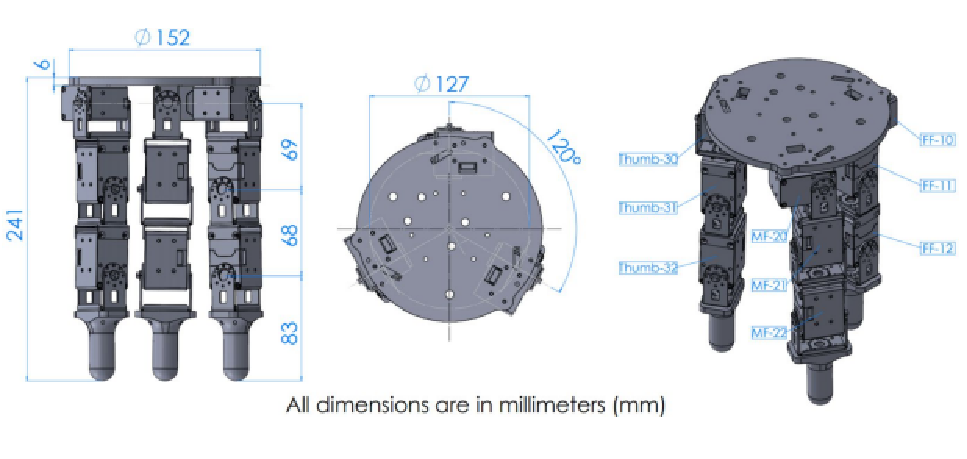
\includegraphics[height=3.5cm]
       {asset/img/dclaw.pdf}
  \caption{D'Clawの概要.FF-10$\sim$Thumb-32までの角度を$\theta^1_{\textrm{j}}\sim\theta^9_{\textrm{j}}$とし,$\boldsymbol{\theta}_{\textrm{j}}=(\theta^1_{\textrm{j}},\cdots,\theta^9_{\textrm{j}})$とおく.また,バルブの角度を$\theta^{\textrm{v}}$のように表記する.\cite{ahn2020robel}より引用.}
  \label{dclaw_structure}
\end{figure}
 
本研究ではオープンソースロボットプラットフォームRobelのハンドロボットD'Clawで実験する\cite{ahn2020robel}.D'Clawの構造は図\ref{dclaw_structure}に示しており,3つの関節を備えた指を3本,合計で9つの関節が存在する.各指の関節の可動域は根元から$27.5^\circ,60^\circ,90^\circ$である.
行動空間は9次元で,各関節の目標角度を可動域の大きさで$[-1,1]$の範囲にスケールしたものを入力とする.状態空間は以下のように関節の角度$\boldsymbol{\theta}^{\textrm{j}}$,関節の角速度$\dot{\boldsymbol{\theta^{\textrm{j}}}}$,バルブの角度の余弦$\textrm{cos}(\theta^{\textrm{v}})$,バルブの角度の正弦$\textrm{sin}(\theta^{\textrm{v}})$,バルブの角度と目標角度の誤差$\theta^{\textrm{v}} - \hat{\theta}^{\textrm{v}}$の合計21次元からなる.
\begin{eqnarray}\label{state}
  s_t = \left(\boldsymbol{\theta}^{\textrm{j}},\dot{\boldsymbol{\theta^{\textrm{j}}}},\textrm{cos}(\theta^{\textrm{v}}),\textrm{sin}(\theta^{\textrm{v}}),\theta^{\textrm{v}} - \hat{\theta}^{\textrm{v}}\right) \nonumber \\ 
\end{eqnarray}

\subsubsection{シミュレーション環境}
このロボットをシミュレーションで学習するにあたって,オープンソースの物理エンジンであるMuJoCoを利用する\cite{Mujoco}.

\subsubsection{実機の設定}
アクチュエータとしてDynamixel XM430-W210を利用する.
%%% 引用:https://emanual.robotis.com/docs/en/dxl/x/xm430-w210/ webサイトを引用する際のbibtexの記載は?




\subsection{実験データの収集}
\subsection{VAEの学習}


\subsection{実験1:同一形状のバルブの学習(シミュレーション)}
・データの存在するものと同一形状のバルブについて学習.
・SACのみ・ファインチューニングと比較.
・Ablation Studyとして,潜在変数の次元を変えて比較.
必要な図表:3種類の条件を比較した図・Ablation studyの図.

\subsection{実験2:異なる形状のバルブへの転移(シミュレーション)}
・データの存在するものと異なる形状のバルブについて学習.
・まず,3本足バルブの方策をそのまま持っていくとどうなるかをまず.
・4種類のバルブについてSACのみ・ファインチューニングと比較.
・Ablation Studyとして,潜在変数の次元を変えて比較.
必要な図表:3本足の方策を4種類のバルブにそのまま持っていったときのバルブの誤差の表・4種類のバルブについて3種類の条件を比較した図・Ablation studyの図.

\subsection{実験3:同一形状のバルブの学習(実機)}
・まず,3本足バルブについてシミュレータで学習した方策をそのまま持っていくとどうなるかをまず.
・SACのみ・ファインチューニングと比較.

\subsection{実験4:異なる形状のバルブへの転移(実機)}
・まず,3本足バルブについてシミュレータで学習した方策をそのまま持っていくとどうなるかをまず.
・4種類のバルブについてSACのみ・ファインチューニングと比較.
必要な図表:3本足の方策を4種類のバルブにそのまま持っていったときのバルブの誤差の表・4種類のバルブについて3種類の条件を比較した図.
実機ならではの図がほしい.



\section{議論}\label{sec-discussion}

\section{結論}\label{sec-conclusion}



%%% 謝辞 %%%%%%%%%%%%%%%%%%%%%%%%%%%%%%%%%%%%%%%%%%%%%%%%%%%%%%%%%%%%%%%%%%%%%%%%
\acknowledgment
に深く感謝する.

%%% 参考文献 %%%%%%%%%%%%%%%%%%%%%%%%%%%%%%%%%%%%%%%%%%%%%%%%%%%%%%%%%%%%%%%%%%%%
\addcontentsline{toc}{section}{\refname} % 目次に参考文献を追加する.
                                         % chapter使用時は削除すること.
\bibliographystyle{junsrt} % jplain.bstの読み込み.
\bibliography{thesis}

%%% BibTeX 等を用いる場合は,上の thebibliography 環境を消してここに該当コードを
%%% 挿入すること.
%% \bibliographystyle{...}
%% \bibliography{...}

%%% 付録 %%%%%%%%%%%%%%%%%%%%%%%%%%%%%%%%%%%%%%%%%%%%%%%%%%%%%%%%%%%%%%%%%%%%%%%%
%%% 付録は不要ならば削除してよい.
\appendix


%%% 本文ここまで %%%%%%%%%%%%%%%%%%%%%%%%%%%%%%%%%%%%%%%%%%%%%%%%%%%%%%%%%%%%%%%%
\fi
\ifoutputcover
\cleardoublepage
%%% 表紙,背表紙,提出用摘要 %%%%%%%%%%%%%%%%%%%%%%%%%%%%%%%%%%%%%%%%%%%%%%%%%%%%
\makecover                      % 表紙
\makespine[\numberofspines]     % 背表紙
\fi
\ifoutputabstractforsubmission
\makeabstractforsubmission      % 提出用摘要
\fi
\end{document}
